%
% Copyright 2018 Markus Borg, Lund University
%
% This work is licensed under a Creative Commons Attribution-ShareAlike 4.0 International License.
% See http://creativecommons.org/licenses/by-sa/4.0/
%
% The dodument is based on a LaTeX template developed by Jean-Philippe Eisenbarth
% https://github.com/jpeisenbarth/SRS-Tex
%
\documentclass{scrreprt}
\usepackage{graphicx}
\usepackage{listings}
\usepackage{underscore}
\usepackage[bookmarks=true]{hyperref}
\usepackage[utf8]{inputenc}
\usepackage[english]{babel}
\hypersetup{
    bookmarks=false,    % show bookmarks bar?
    pdftitle={Lab 3},    % title
    pdfauthor={Markus Borg},                     % author
    pdfsubject={TeX and LaTeX},                        % subject of the document
    pdfkeywords={TeX, LaTeX, graphics, images}, % list of keywords
    colorlinks=true,       % false: boxed links; true: colored links
    linkcolor=blue,       % color of internal links
    citecolor=black,       % color of links to bibliography
    filecolor=black,        % color of file links
    urlcolor=purple,        % color of external links
    linktoc=page            % only page is linked
}%
\def\myversion{0.2 }
\date{}
%\title
\usepackage{hyperref}
\begin{document}

\begin{flushright}
    \rule{16cm}{5pt}\vskip1cm
    \begin{bfseries}
    	\LARGE{ETSA02-ADM-LAB2}\\
    	\vspace{1.5cm}
        \Huge{Lab 3}\\
        \vspace{0.5cm}
        System testing\\
        \vspace{0.5cm}
        in Robocode\\
        \vspace{1.5cm}
        \LARGE{Version \myversion approved}\\
        \vspace{1.5cm}
        Prepared by Markus Borg\\
        %\vspace{1.5cm}
        Dept. of Computer Science, Lund University\\
        \vspace{1.5cm}
        \today\\
    \end{bfseries}
\end{flushright}

%\tableofcontents

\chapter*{Revision History}

\begin{center}
    \begin{tabular}{|c|c|c|c|}
        \hline
	    Name & Date & Reason For Changes & Version\\
        \hline
	    Markus Borg & 2018-03-21 & Initial draft. & 0.1\\
        \hline
        Markus Borg & 2018-04-01 & First instructions for the RobotTestBed. & 0.2\\
        \hline
    \end{tabular}
\end{center}

\chapter{Introduction}
System testing.\\
Testing of quality requirements.

\chapter{Before the lab}
Just like for Lab 2 you will find the code required for this lab on GitHub: https://github.com/lunduniversity/introsofteng
If you have already cloned the repository, pull the latest source code to make sure you work with the latest version. If you prefer downloading the code, instead click the button presented in Figure~\ref{fig:github} and choose ``Download ZIP''. For Lab 3, you need the files located in introsofteng-master/project/rumble/labs/lab3/src, including its subfolder: `test'. Rewatch the video ``Lab2_download.avi'' on Google Drive (ETSA02 Everyuone/Labs) if you need support.

\begin{figure}
\centering
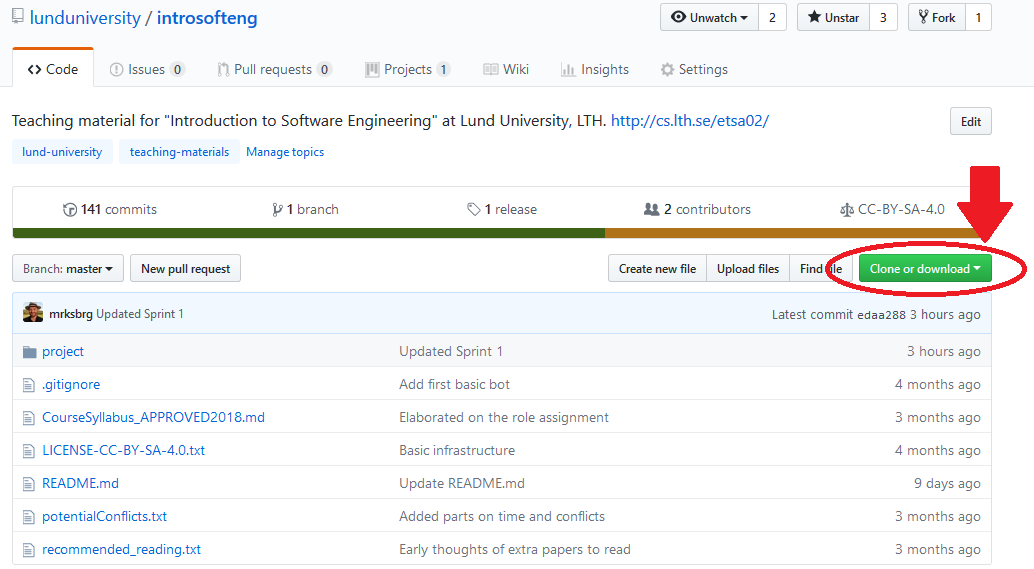
\includegraphics[width=0.99\textwidth]{figures/GitHub.png}
\caption{introsofteng repository on GitHub. The arrow shows the ``Clone or download'' button.}
\label{fig:github}
\end{figure}

%Download the latest Robot testing plugin (1.9.3.0) from http://robo-code.blogspot.se/\\
%Add robocode.testing.jar to the Java build path in Eclipse\\
%Create a run configuration for JUnit in Eclipse\\
%Add -Drobocode.home=$<$PATH TO ROBOCODE$>$ as an argument to the VM\\
%Might need to configure Eclipse project: Properties -> Java Build Path -> Libraries -> Add Library -> JUnit -> Junit 5\\
%Try running JUnit tests

\chapter{At the lab}

%Select your robot class in the Eclipse package explorer. Right-click and select new JUnit test case. Create the new test case. There are several naming conventions, e.g., using the same name as the class under test followed by the suffix `Test' and `Test' as prefix for all methods.
%Software-under-test is the normal name for the object to test, here we use bot-under-test.\\
%Introduce test driven development.

%Inspiration: https://ics613s13.wordpress.com/\\
%Build a robot using maven: https://github.com/bretkikehara/robocode-bki-hunter

%\section{Install Robocode}
%Download latest Robocode: https://sourceforge.net/projects/robocode/files/\\
%Install on local drive\\
%Start a few battles. Experiment.\\
%Develop a quick robot using the internal editor: http://robowiki.net/wiki/Robocode/My_First_Robot\\
%Compile it and try it in battles.
%
%\section{Develop a Robot in Eclipse} \label{sec:develop}
%Create a project in Eclipse http://robowiki.net/wiki/Robocode/Eclipse/Create_a_Project\\
%Download the Basic Leader Bot to the project. Make sure it builds.
%
%\section{Try the robot in Robocode} \label{sec:try}
%Add the Robot project in Robocode: http://robowiki.net/wiki/Robocode/Add_a_Robot_Project\\
%Note: Add the path to the Eclipse project (with /src and /bin as sub-folders), not the workspace.
%
%\section{Configure Eclipse to run and debug the robot}
%Run from Eclipse: http://robowiki.net/wiki/Robocode/Eclipse/Running_from_Eclipse\\
%Set up debugging from Eclipse: http://robowiki.net/wiki/Robocode/Eclipse/Debugging_Robot
%
%\section{Expand the team} \label{sec:expand}
%Repeat the instructions in Sections~\ref{sec:develop}-\ref{sec:expand} for the Basic Bot and the Basic Drone.\\
%Create a team from within Robocode (Robot-$>$Create a robot team)\\
%Try a few team battles against various opposition.

\chapter{After the lab}
%Reflect on what is important for successful team battles. Consider your two perspectives. First, think about what type of team you want to build to be run a successful LU rumble.
%
%Second, discuss what type of Robot you want to release on the market. What types will be in high demand? What is the competition going to offer? What could be your niche? Think about commodity, differentiation, and innovation.
%
%Successful development of software products for an open market requires making critical decisions under time pressure -- decisions of both technical nature as well as business nature. Your team needs to decide soon!

\end{document}
